\documentclass[lettersize,journal]{IEEEtran}
\usepackage{amsmath,amsfonts,amssymb}
\usepackage{array}
\usepackage{textcomp}
\usepackage{stfloats}
\usepackage{url}
\usepackage{verbatim}
\usepackage{graphicx}
%\usepackage[caption=false,font=normalsize,labelfont=sf,textfont=sf]{subfig}
\usepackage{caption}
\captionsetup[figure]{font=footnotesize,labelfont=footnotesize,textfont=footnotesize,labelsep=period}
\usepackage{subcaption}

\usepackage{cite}
\usepackage{tabularx}
\usepackage{gensymb}  
\usepackage{enumitem}
\usepackage{hyperref}
\usepackage{booktabs}

\usepackage{algorithm}
\usepackage{algpseudocode}  % proporciona \begin{algorithmic}[1] … \end{algorithmic}
\usepackage{xfrac}

\newtheorem{remark}{Remark}[section] % declara el entorno “remark”

\begin{document}

\title{Beam-Steered Single-LED Single-PD Visible-Light Positioning for 3D Localization}
\author{Author~Name,~\IEEEmembership{Member,~IEEE,} and Second~Author,~\IEEEmembership{Senior~Member,~IEEE}% 
\thanks{ The authors are with the Laboratoire d’Ingénierie des Systèmes de Versailles (LISV), Université of Paris-Saclay, UVSQ, 78140
 Vélizy-Villacoublay, France (e-mail: aaaaa@uvsq.fr; aaaaa@uvsq.fr; aaaaa@uvsq.fr; aaaaa@uvsq.fr).}
}
\markboth{Journal of \LaTeX\ Class Files,~Vol.~14, No.~8, August~2021}%
{Shell \MakeLowercase{\textit{et al.}}: A Sample Article Using IEEEtran.cls for IEEE Journals}
%\IEEEpubid{0000--0000/00\$00.00~\copyright~2021 IEEE}
\maketitle

\begin{abstract}
\end{abstract}

\begin{IEEEkeywords}
    VLP, Single LED VLP, CRLB, 3D positioning, GLS
\end{IEEEkeywords}

% *******************************************
\section{Introduccion}
% *******************************************
\begin{itemize}
    \item K es el número total de orientaciones
    \item N es el número total de muestras por cada orientación
    \item C es la constante optica.
\end{itemize}



% *******************************************
\section{System Model}
\label{sec:System Model}
% *******************************************
En la Figura 1 se muestra el diagrama del sistema VLP a estudiar. El sistema está compuesto por un transmisor LED posicionado en el techo a una altura H, $\mathbf{T}=(0,0,H)$, cuyo vector de orientación $\mathbf{n_t}$ es modulable; el receptor es un unico fotodiodo orientado verticalmente $\mathbf{n_r}=(0,0,1)$, de posición desconocida en el espacio tridimensional $\mathbf{R}=(x,y,z)$. Asimismo se denomina $\mathbf{d}$ como el vector distancia entre el transmisor y el receptor $(\mathbf{d} = R - T)$.

Para la $i$-th orientación del transmisor de potencia $P_t$, la potencia recibida en el receptor es:

\begin{equation}
P_{r}^{(i)} = P_t\,h_{\mathrm{LOS}}^{(i)} + \eta^{(i)},
\label{eq:received_power}
\end{equation}

donde $\eta$ es el zero-mean additive white Gaussian noise $\mathcal N(0,\sigma^2)$ y $h_\mathrm{LOS}$ es la ganancia del canal óptico definido por el modelo lambertiano:

\begin{equation}
h_{\mathrm{LOS}} =
\begin{cases}
\dfrac{(m+1)A_{\mathrm{det}}}{2\pi d^{2}}\;\cos\phi_i^{m}\,\cos\psi, & \psi \le \Psi_{\mathrm{FOV}},\\[6pt]
0,&\text{otherwise},
\end{cases}
\label{eq:h_los}
\end{equation}

donde $m=\frac{-\ln 2}{\ln(\cos\Phi_{1/2})}$ es el orden lambertiano asociado al LED half-power angle $\Phi_{1/2}$, $A_{\mathrm{det}}$ es el área efectiva del fotodiodo, $\phi$ y $\psi$ son los angulo de irradiancia e incidencia respectivamente, $\Psi_{\mathrm{FOV}}$ is the receiver field of view, $d$ la distancia transmisor receptor. Además, el coseno de los angulos de irradianza y de incidencia se pueden calcular como:
\begin{equation}
    \cos\phi_i = \frac{\mathbf{n_{t}}^{(i)}\;\cdot\mathbf{d}}{d},
    \qquad    
    \cos\psi   = \frac{\mathbf n_{r}\;\cdot(-\mathbf{d})}{d}.
\label{eq:cosenos}
\end{equation}


Por cada orientación se registran $N$-muestras en el receptor. El estimador eficaz de la potencia recibida en cada $i$-th orientación considerando el comportamiento de ruido gaussiano es la estadística siguiente:
\begin{equation}
    P_r^{(i)}=\frac{1}{N}\sum_{j=1}^{N}{P_{r,j}^{(i)}}\;,\; P_r^{(i)}\sim \mathcal N(\mu,\frac{\sigma^2}{N})
    \label{eq:promedios}
\end{equation}
la que consideraremos como potencia recibida promedio.

Ademas, definiremos el SNR*(dB) promedio de un testbed como el $10\log_{10}(\overline{\mathrm{SNR}}_{r}^{(i)})$, donde $\overline{\mathrm{SNR}}_{r}^{(i)}$ es el promedio de todos los $\mathrm{SNR}_{r}^{(i)}$ de una posición $r \in \mathrm{testbed}$ a una orientacion i=1,2,...,K del transmisor y se calcula como:
\begin{equation}
\mathrm{SNR}_{r}^{(i)}=\frac{P_t\,h_{\mathrm{LOS}}^{(i)}}{\sigma^2}
\end{equation}


\begin{figure}[t]
    \centering
    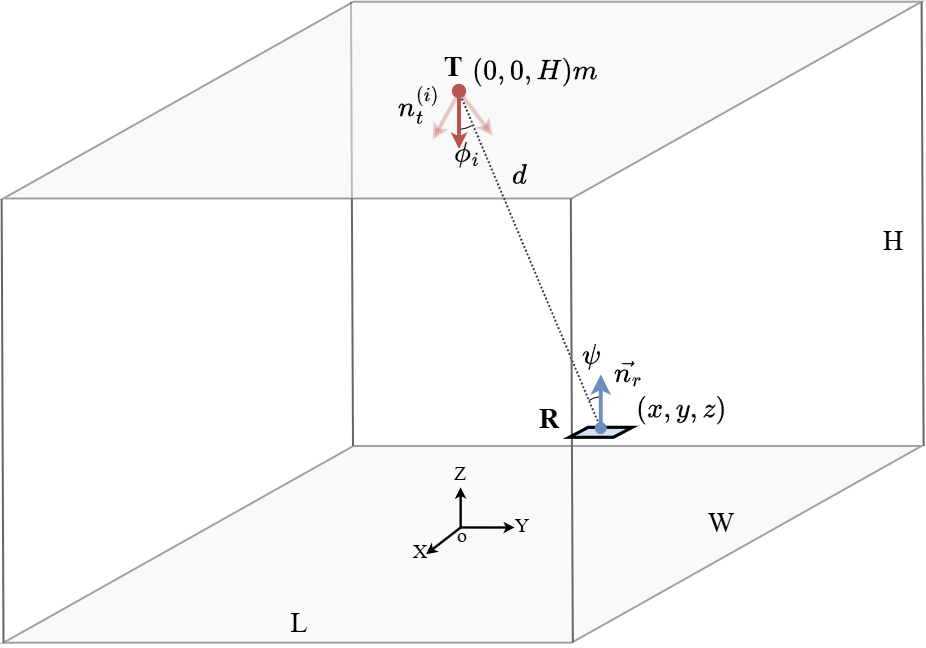
\includegraphics[width=\linewidth]{Figures/II. System/system.png}
  \caption{Configuration of the system Single LED Visible Light Positioning.}
    \label{fig:system}
\end{figure}



% *******************************************
\subsection{Método general de estimacion de posicion 3D Single LED}
% *******************************************
\subsubsection{Vector de direction finding}
En este primer paso se estima la dirección del transmisor para apuntar hacia el Receptor. E ste es un vector unitario que se relaciona con el vector distancia $\mathbf{n_d}=\frac{\mathbf{d}}{\lVert \mathbf{d} \rVert}$. Para determinar la dirección se modula la orientación del transmisor K-veces. En las secciones \ref{sec:NoLineal} y \ref{sec:Lineal} se exploran diferentes métodos model-based para su estimación.

\subsubsection{Distance recovery}
Empleando la estimación de la dirección, reorientamos al Transmisor con $\mathbf{n_t}=\mathbf{\hat n_d}$, manteniendose en un escenario beamstearing, sin perder generalización, asumimos que podemos reorientar el receptor y lo reorientamos para que apunte al transmisor con $\mathbf{n_r}=-\mathbf{\hat n_d}$ con la finalidad de maximizar la potencia recibida promedio. Se registran N muestras y se determina la distancia.

Considerando este alimentamiento, asumiendo que la constante 
\begin{equation}
    C=\frac{P_t(m+1)A_{\det}}{2\pi},   
    \label{eq:constante_optica}
\end{equation}
es conocida o calculada mediante calibración previa y empleando las ecuaciones eq.\eqref{eq:received_power}\eqref{eq:h_los}\eqref{eq:cosenos} se puede determinar que 

\begin{equation}
\mu^* = \frac{C}{d^2}
\label{eq:relacion_distance}
\end{equation}

donde $\mu^*$ es una muestra de la potencia recibida en este escenario. En la práctica, $N$ independent samples $\{\mu^{*}_j\}_{j=1}^N$ are collected under this beamsteered configuration. Siguiendo la eq.\eqref{eq:promedios} se determina $\hat\mu^*=\frac{1}{N}\sum_{j=1}^N \mu^{*}_j \;\sim\; \mathcal N\Bigl(\mu^*,\,\sigma^2/N\Bigr)$. Substituting $\hat\mu^*$ into~\eqref{eq:relacion_distance} y despejando la distancia tenemos:
\begin{equation}
  \hat d  =  \sqrt{\frac{C}{\hat\mu^*}}.
  \label{eq:range_estimate}
\end{equation}

La posición 3D estimada es:
\begin{equation}
  \hat{\mathbf R} 
  \;=\; 
  \mathbf T + \hat d \,\hat{\mathbf n}_d.
  \label{eq:Rhat_full}
\end{equation}

% *******************************************
\section{Position Error Bound}
\label{sec:PEB}
% *******************************************
% Fundamento matemático y descripción del PEB. Mencionar que es ampliamente empleado para optimización de parámetros y evaluación de que tan bien está un estimador propuesto.
% Expresion homeodastica de las K+1 ecuaciones con ruido gaussiano independiente. Cada PDF es una función gaussiana. Son K+1 ecuaciones porque hay K ecuaciones para la estimación del vector de dirección y 1 ecuacion para distance Recovery. Cada ecuación proviene de la potencia promedio en esa orientación determinada (eq.\ref{eq:promedios})
% Definir la función L de likelihood y log-likelihood.
% Determinar la Matriz de información de fisher (FIM) denotada con la variable I(theta). Normalmente se emplea -E[ gradiente_theta^2 {ln(L(theta))}] pero también se puede calcular como varianza del score I(θ)=Var[∇θ ℓ(θ)]=E[(∇ θ ℓ)(∇ θ ℓ)T]. Justificar porque se usa esta ultima.
% Definir finalmente el PEB en términos de I(theta).


En esta sección se desarrolla la Position Error Bound (PEB), la cota inferior de Cramér–Rao (CRLB) aplicada al vector de posición, la cual determina la varianza mínima alcanzable por un estimador insesgado de la posición $\mathbf R=(x,y,z)^{\mathsf T}$ en el sistema propuesto. En este trabajo el PEB es empleado como métrica de referencia para cuantificar qué tan cercano al óptimo se situa un estimador específico y métrica para la optimización de parámetros del diseño que minimicen el error de posicionamiento.

\subsection{Modelo estadístico conjunto de las observaciones}

De acuerdo con la Sección~\ref{sec:System Model}, para cada una de las $K$ orientaciones del transmisor se calcula la potencia promedio
\[
P_r^{(i)} \sim \mathcal N\!\bigl(\mu_i(\mathbf R),\sfrac{\sigma^2}{N}\bigr), 
\qquad i\!=\!1,\dots,K,
\]
donde 
\(
\mu_i(\mathbf R)=P_t \, h_{\mathrm{LOS}}^{(i)}(\mathbf R)
\)
y $h_{\mathrm{LOS}}^{(i)}(\mathbf R)$ se define en~\eqref{eq:h_los} con los cosenos dados en~\eqref{eq:cosenos}.  
Adicionalmente, tras la etapa de \emph{beam‑steering} se obtiene la estadística de \emph{distance‑recovery}
\[
\mu^{*}\sim\mathcal N\!\bigl(C/d^{2}(\mathbf R),\sfrac{\sigma^2}{N}\bigr),
\]
en la que $d(\mathbf R)=\lVert\mathbf R-\mathbf T\rVert$ y la constante $C$ se definió en~\eqref{eq:constante_optica}.  

Agrupando todas las $(K+1)$ variables aleatorias se define el vector de mediciones

\[
\mathbf z
=
\begin{bmatrix}
P_r^{(1)} & \!\dots & P_r^{(K)} & \mu^{*}
\end{bmatrix}^{\!\mathsf T}
\sim 
\mathcal N\!\bigl(\boldsymbol\mu(\mathbf R),\;\mathbf\Sigma\bigr),
\]

donde 
\(
\boldsymbol\mu(\mathbf R)=
\bigl[\mu_1(\mathbf R),\dots,\mu_K(\mathbf R),\mu_{K+1}(\mathbf R)\bigr]^{\mathsf T}
\)
y la matriz de covarianza es diagonal, $\mathbf\Sigma=\frac{\sigma^2}{N}\,\mathbf I_{K+1}$, gracias a la independencia de las mediciones y a la media muestral empleada en~\eqref{eq:promedios}.

\subsection{Función de log-verosimilitud y score}
Considerando independencia entre las mediciones, la función de verosimilitud es el producto de $(K+1)$ densidades gaussianas idénticamente distribuidas. El principio de máxima verosimilud para determinar la estimador eficaz se mantiene si se realiza a partir del logaritmo-verosimilitud, más conveniente para el cálculo, el cual se calcula como:

\begin{equation}
\ell(\mathbf R) = \ln L(\mathbf R\,|\,\mathbf z) = -\frac{N}{2\sigma^{2}}\sum_{i=1}^{K+1}\bigl[z_i-\mu_i(\mathbf R)\bigr]^2+\text{cte}.
\label{eq:loglike}
\end{equation}

El vector \emph{score} se define como el gradiente de~\eqref{eq:loglike} respecto de los parámetros de interés:

\[
\mathbf s(\mathbf R)
=
\nabla_{\mathbf R}\ell(\mathbf R)
=
\frac{N}{\sigma^{2}}
\sum_{i=1}^{K+1}
\bigl[z_i-\mu_i(\mathbf R)\bigr]\,
\nabla_{\mathbf R}\mu_i(\mathbf R),
\]
donde 
\(
\nabla_{\mathbf R}=\bigl[\partial/\partial x,\;
\partial/\partial y,\;
\partial/\partial z\bigr]^{\!\mathsf T}.
\)

\subsection{Matriz de Información de Fisher}

Para distribuciones pertenecientes a la familia exponencial, tal como la gaussiana homocedástica de este trabajo, la Fisher Information Matrix (FIM) puede calcularse como la varianza del score, lo cual evita la diferenciación de segundo orden y resulta numéricamente más estable:

\begin{align}
\mathbf I(\mathbf R)
&\;=\;\operatorname{Var}\!\bigl[\mathbf s(\mathbf R)\bigr]
= \mathbb E_{\mathbf z}\!
\bigl[\mathbf s(\mathbf R)\,\mathbf s^{\mathsf T}(\mathbf R)\bigr] \\
&\;=\;
\frac{N}{\sigma^{2}}
\sum_{i=1}^{K+1}
\bigl[\nabla_{\mathbf R}\mu_i(\mathbf R)\bigr]\,
\bigl[\nabla_{\mathbf R}\mu_i(\mathbf R)\bigr]^{\!\mathsf T}.
\label{eq:FIM_general}
\end{align}

La última igualdad se obtiene usando que $\mathbb E[z_i]=\mu_i(\mathbf R)$, de modo que $\mathbb E\bigl[(z_i-\mu_i)(z_j-\mu_j)\bigr]=0$ cuando $i\neq j$.  La información total es, por tanto, la superposición coherente de las contribuciones diferenciales de cada orientación y de la medida de distancia.

\paragraph*{Gradientes necesarios}

\begin{enumerate}
\item
Para la $i$‑ésima orientación,
\[
\nabla_{\mathbf R}\mu_i(\mathbf R)
=
P_t\nabla_{\mathbf R}h_{\mathrm{LOS}}^{(i)}(\mathbf R),
\]
siendo necesario derivar~\eqref{eq:h_los} empleando la regla de la cadena sobre $d(\mathbf R)$, $\cos\phi_{i}$ y $\cos\psi$, resultando en:

\begin{multline}
\nabla_{\mathbf R}\mu_i(\mathbf R) =
\frac{C}{d^{3}}
\Bigl[
m\cos^{m-1}\!\phi_i\;\cos\psi\;\mathbf n_t^{(i)}
\;-\;\\
\cos^{m}\!\phi_i\,\mathbf n_r
\;-\;
(m+3)\cos^{m}\!\phi_i\;\cos\psi\;\mathbf n_d
\Bigr],
\label{eq:grad_mu_closed}
\end{multline}
%\qquad \psi\le\Psi_{\mathrm{FOV}}.
%\tag{PEB‑G1}

para $\psi>\Psi_{\mathrm{FOV}}$ se anula el gradiente porque $h_{\text{LOS}}^{(i)}=0$.




\item
Para la ecuación de \emph{distance‑recovery},
\begin{equation}
    \nabla_{\mathbf R}\mu_{K+1}(\mathbf R)
=
-\,\frac{2C}{d^{4}} 
\bigl(\mathbf R-\mathbf T\bigr)
=
-\,\frac{2C}{d^{3}}\,
\mathbf n_d,
\end{equation}

donde $\mathbf n_d$ es el vector unitario definido en la Sección~II‑A.
\end{enumerate}

\subsection{Definición formal del PEB}

Sea $\hat{\mathbf R}$ cualquier estimador insesgado de $\mathbf R$.  El teorema de Cramér–Rao establece

\[
\operatorname{Cov}\!\bigl[\hat{\mathbf R}\bigr] 
\succeq 
\mathbf I^{-1}(\mathbf R),
\]

por lo que una medida escalar de desempeño PEB se define como

\begin{equation}
\text{PEB}(\mathbf R)
=\sqrt{\operatorname{tr}\bigl\{\mathbf I^{-1}(\mathbf R)\bigr\}}\;.
\label{eq:PEB}
\end{equation}

La raíz de la traza de la inversa de la FIM representa la \emph{desviación estándar cuadrática mínima} (RMSE) que cualquier sistema VLP con las $K+1$ mediciones descritas podría alcanzar en la estimación de posición.  Una PEB pequeña implica que el conjunto de orientaciones elegido y la medición de rango aportan información suficiente y complementaria para localizar el receptor con alta precisión; en cambio, una PEB grande sugiere la necesidad de aumentar $K$, mejorar la relación señal‑a‑ruido, o rediseñar el patrón de orientaciones.

%-------------------------------------------------------------------------------
\subsection{Number of orientations}
%-------------------------------------------------------------------------------

\paragraph{$K\le2$ } (sub–determined)
\paragraph{$K=3$ } (just–determined)
\paragraph{$K\ge 4$ } (over–determined)



% *******************************************
\section{Optimization of set of orientations}
\label{sec:optimization}
% *******************************************
Como se puede apreciar en la eq. \ref{eq:grad_mu_closed} el set de K orientaciones $\mathbf{n_t^{(i)}}$ impacta en la FIM, que a su vez impacta en la PEB. Por lo que es importante encontrar un set óptimo de orientaciones que minimice el PEB. Debido a la naturaleza no lineal de la función PEB, encontrar $\mathbf{n_t^{(i)}}$ tal que $\mathbf{n_t^{(i)}}=argmin(PEB)$ no es trivial. En el presente trabajo se propone el uso de algoritmos genéticos para la busqueda del set de orientaciones óptimo para diferentes K que minimice el PEB global.

Los algoritmos genéticos se inspiran en la selección natural de darwin. Una población es generada aleatoriamente, se evalua basado en una determinada métrica, los mejores sujetos denominados progenitores son seleccionados y cruzados, mientras que se añade a la población una tasa de individuos con mutación a fin de agregar variabilidad para no caer en minimos locales; el proceso se repite por un número determinado de generaciones máxima. En el contexto de nuestro problema, los individuos tiene como características un set de K-orientaciones unitarias, cada vector de orientación es definido por completo con su angulo de elevación y azimuth $(\theta_i,\rho_i)$ el cual es equivalente a su vector unitario $n_t^{(i)}=(\sin(\theta_i)\cos(\rho_i),\sin(\theta_i)\sin(\rho_i),-\cos(\theta_i))$. Es decir, para un set de $K$ orientaciones, un individuo posee $2K$ características: $(\theta_1,\rho_1,\theta_2,\rho_2,...,\theta_K,\rho_K)$. La métrica de evaluación es el 90-percentil del $\mathrm{PEB}$ (es decir  $\mathrm{PEB_{90\%}}$) obtenido al evaluar en cada posición del recentor la eq.\ref{eq:PEB} dentro de un grillado tridimensional que compone el testbed 3D. El algoritmo genético fue implementado en MATLAB y los parámetros empleados para la optimización se muestran en la tabla \ref{tab:ga_params}.


\begin{table}[ht]
\centering
\caption{Parámetros empleados en la optimización por algoritmo genético}
\label{tab:ga_params}
%\scriptsize
%\setlength{\tabcolsep}{6pt}
\begin{tabular}{|l|l|}
\hline
\multicolumn{2}{|c|}{\textbf{Parámetros del sistema}} \\ \hline
\textbf{Parámetro} & \textbf{Valor} \\ \hline
Posición del transmisor           & $T=(0,0,2)\,$m \\ \hline
Potencia óptica transmitida       & $P_t=0.405\,$W \\ \hline
Ángulo semipotencia (half‐power)  & $\Phi_{1/2}=45^\circ$ \\ \hline
Orden Lambertiano                 & $m=-\ln2/\ln(\cos45^\circ)=2$ \\ \hline
Área efectiva del fotodiodo       & $A_{\mathrm{det}}=4.8\times5.5\,\mathrm{mm}^2$ \\ \hline
FOV del receptor                   & $\Psi_{\mathrm{FOV}}=85^\circ$ \\ \hline
Varianza de ruido por muestra     & $\sigma^2=10^{-21}\times30\times10^6\ \mathrm{W}^2$ \\ \hline
Muestras por orientación          & $N=1000$ \\ \hline
\multicolumn{2}{|c|}{\textbf{Algoritmo genético}} \\ \hline
\textbf{Parámetro} & \textbf{Valor} \\ \hline
Población inicial                 & 300 \\ \hline
Generaciones máximas              & 200 \\ \hline
Fracción de crossover             & 0.8 \\ \hline
Rango permitido de valores        & $\theta_{i} \in [0,80^\circ], \rho_{i} \in [0,360^\circ]$ \\ \hline
Métrica de optimización           & RMS \\ \hline
Parámetros a optimizar            & $[\theta_{1},\rho_{1},\dots,\theta_{K},\rho_{K}]$ \\ \hline
\multicolumn{2}{|c|}{\textbf{Test‐bed 3D}} \\ \hline
\textbf{Parámetro} & \textbf{Valor} \\ \hline
Room dimension LxWxH              & $3\times 3 \times 2\; (\mathrm{m^3})$ \\ \hline
Rango en $x,y$                    & $[-1.5,\,1.5]\,$m \\ \hline
Rango en $z$                      & $[0,\,1.2]\,$m \\ \hline
Paso de malla                     & $0.2\,$m \\ \hline
\end{tabular}
\end{table}

\begin{table*}[ht]
\centering
\caption{Orientaciones óptimas \((\theta_i,\rho_i)\) en grados para distintos valores de \(K\) para un room de $3\times 3 \times 2\; (\mathrm{m^3})$.}
\label{tab:optimal_orientations_2col}
\begin{tabular}{c*{10}{>{\centering\arraybackslash}p{1.2cm}}}
\toprule
\(K\) 
    & \(i=1\)       & \(i=2\)       & \(i=3\)       & \(i=4\)       & \(i=5\)       & \(i=6\)       & \(i=7\)       & \(i=8\)       & \(i=9\)       & \(i=10\)      \\
\midrule
3   & (35.4,140.1)  & (33.3,36.4)   & (29.6,262.7)  &               &               &               &               &               &               &               \\
4   & (38.9,90.6)   & (41.5,0.1)    & (41.8,180.1)  & (38.8,270.2)  &               &               &               &               &               &               \\
5   & (0.1,211.1)   & (50.7,180.0)  & (50.4,359.9)  &  (50.6,90.0)  & (50.6,270.0)  &               &               &               &               &               \\
6   & (17.2,306.9)  & (54.5,266.1)  & (22.5,140.4)  & (52.2,360.0)  & (52.4,84.0)   & (55.8,185.2)  &               &               &               &               \\
7   & (58.9,355.7)  & (53.8,170.7)  & (27.8,43.8)   & (5.4,305.9)   & (54.4,96.5)   & (35.1,220.0)  & (54.8,278.6)  &               &               &               \\
8   & (51.8,89.4)   & (61.5,268.3)  & (27.3,317.0)  & (6.5,318.3)   & (57.8,5.8)    & (53.7,171.3)  & (38.0,200.3)  & (39.3,91.1)   &               &               \\
9   & (56.9,178.7)  & (36.5,266.8)  & (33.9,182.3)  & (2.5,28.2)    & (42.2,78.4)   & (53.1,97.5)   & (57.9,359.7)  & (37.1,355.1)  & (58.2,272.1)  &               \\
10  & (56.0,3.6)    & (53.2,182.5)  & (54.9,356.8)  & (11.9,38.1)   & (61.3,270.3)  & (50.2,91.3)   & (47.6,174.7)  & (43.4,89.4)   & (32.5,277.6)  & (15.1,255.3)  \\
\bottomrule
\end{tabular}
\end{table*}

La tabla \ref{tab:optimal_orientations_2col} muestra el set de K-orientaciones optimos para los parámetros de la tabla \ref{tab:ga_params}, cada set de $K$-orientaciones es distino y ningun set es subconjutos de otro. Por cada set óptimo se determina el PEB o RMS de cada posición de R dentro del testbed, la distribución y grafico de box se muestran de color verde en la figura \ref{fig:Optimized_vs_Random}, comparativamente se realiza el mismo procedimiento con un set de orientaciones random; confirmamos que la distribución de RMS con el set óptimo presenta mejores medidas estadísticas que con un set random, además la mediana de esta distrubución se reduce conforme se aumenta el número de K en el caso del set óptimo. La figura \ref{fig:optimo_vs_random_3D} muestra la distrubición espacial del PEB de la estimación del error en las posiciones del receptor dentro del testbed 3x3 a una altura de 0.8m empleando K=5 orientacioens con el transmisor en el centro; en el set óptimo Fig. \ref{fig:optimo_vs_random_3D}(a) los errores se incrementan en los bordes y especialmente en las esquinas, similar al comportamiento de un sistema tradicional con multi-transmisor, estos errores se distribuyen uniformemente; a diferencia de un set-no optimo donde los errores los mayores y no uniformes.

\begin{figure}[tb]
    \centering
    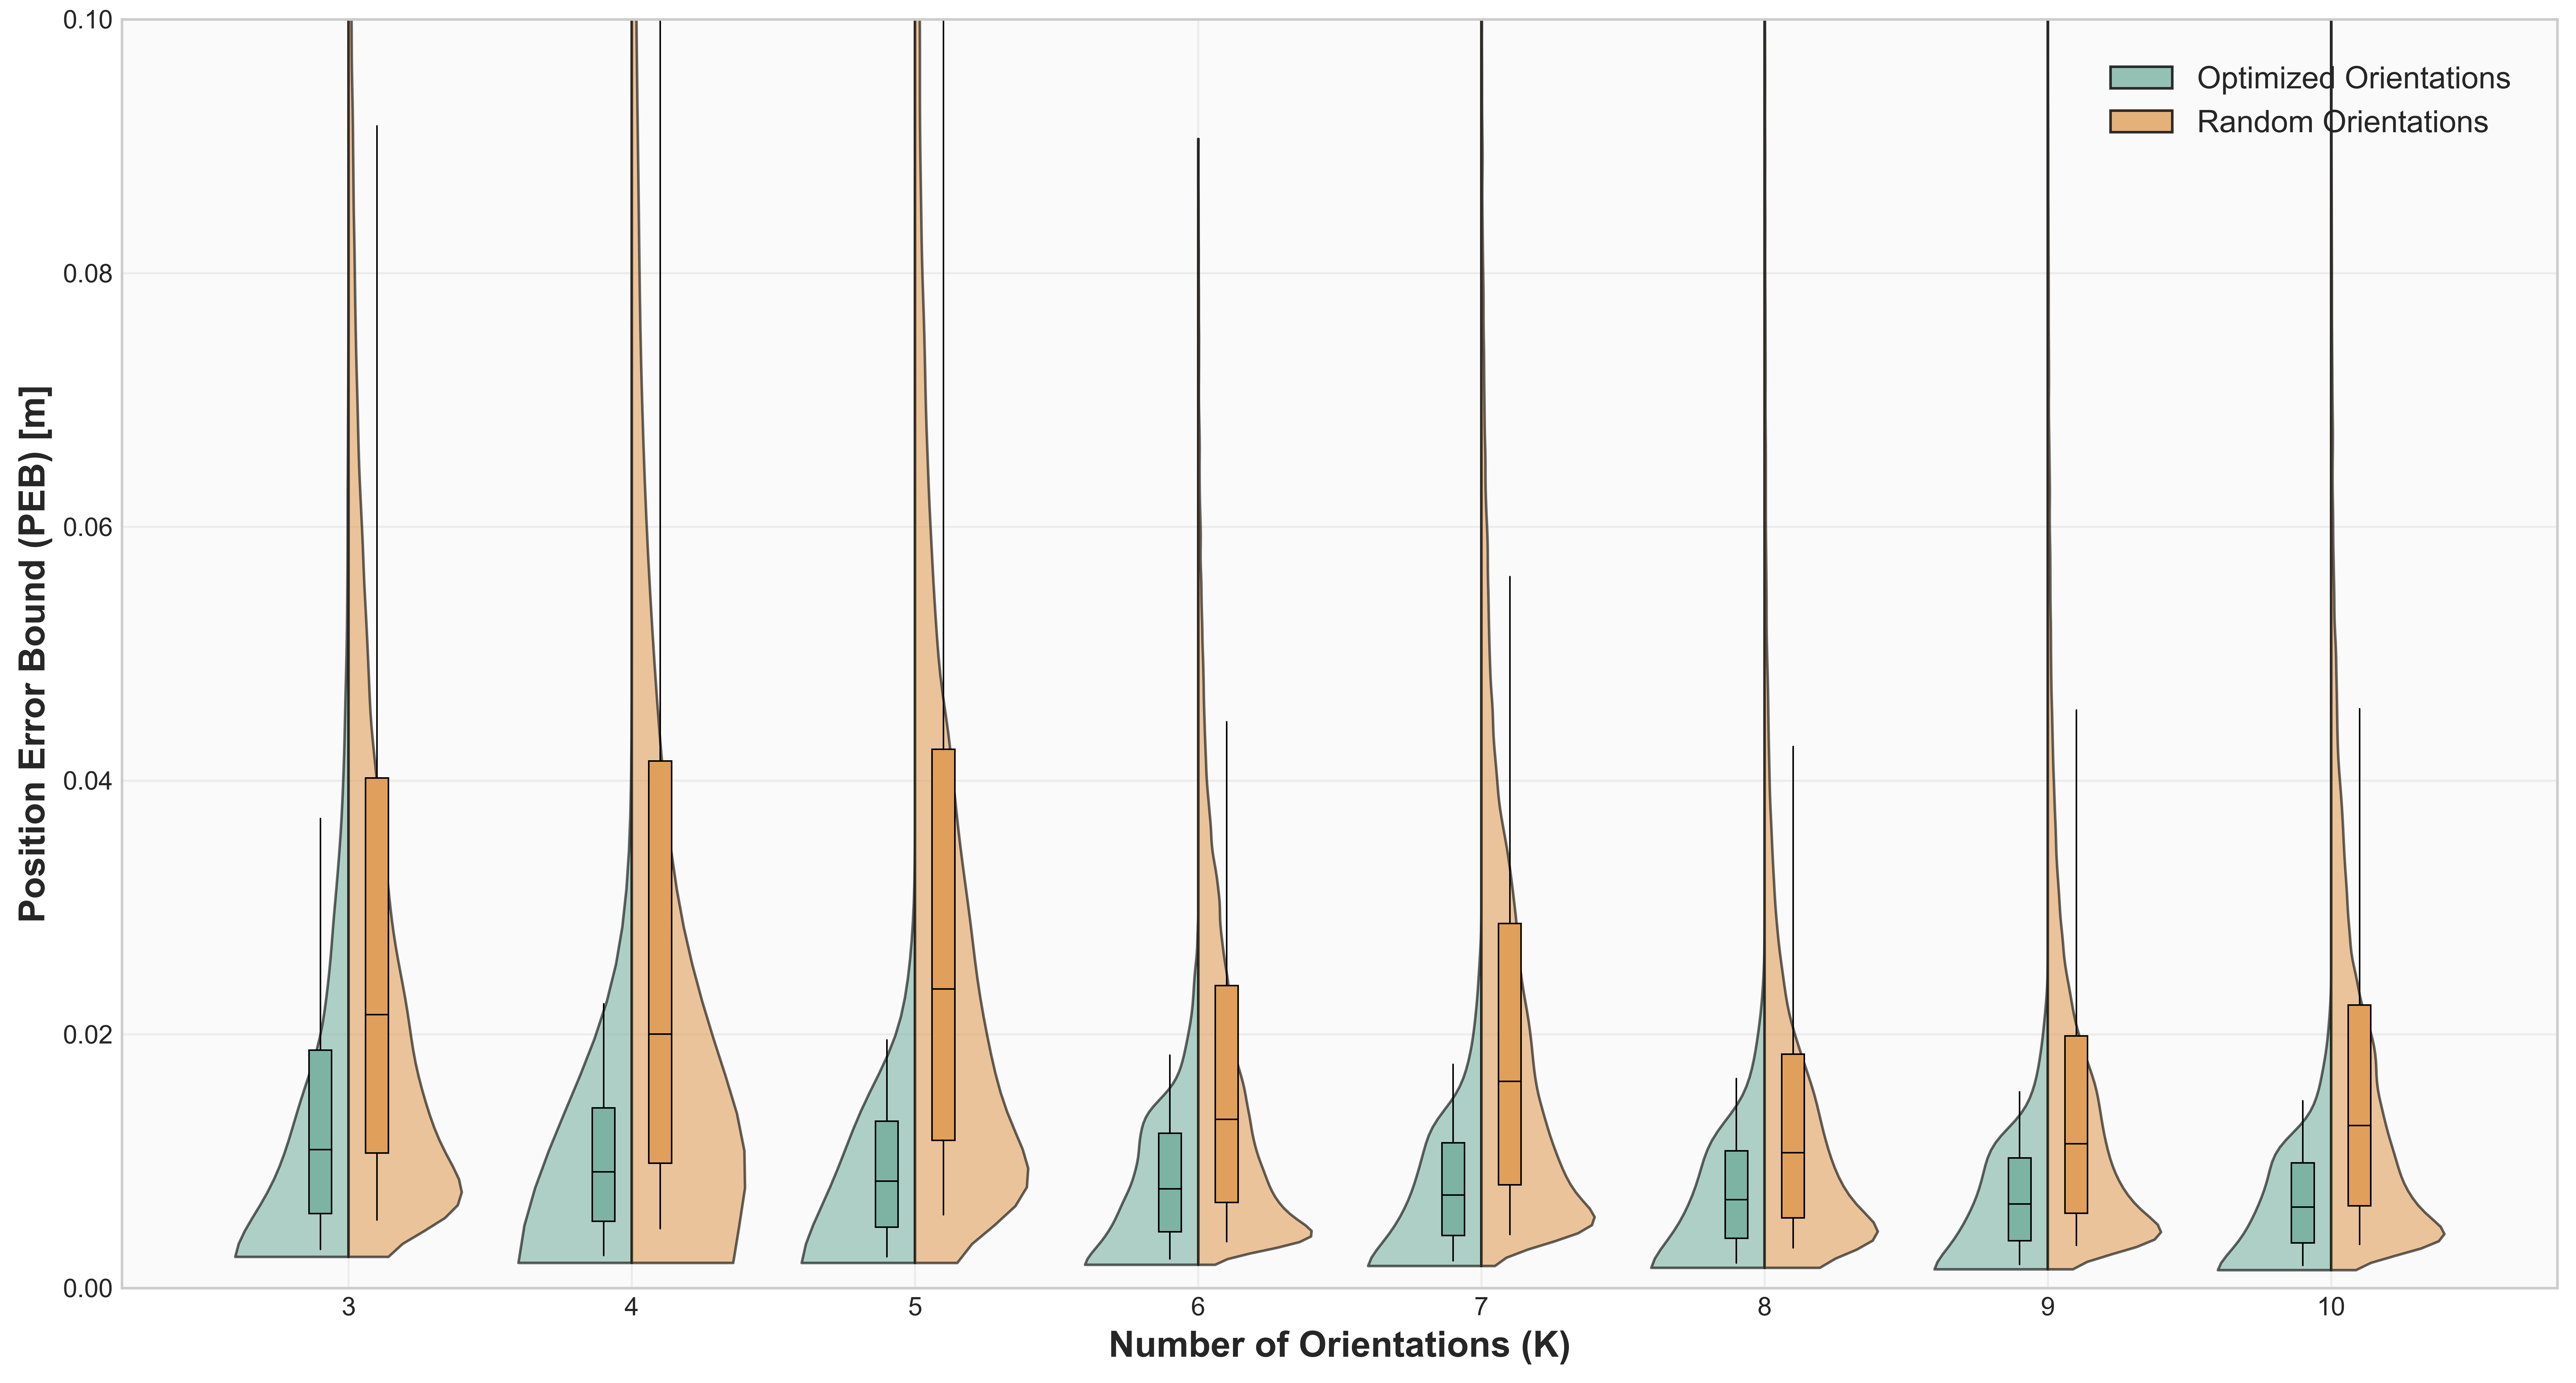
\includegraphics[width=\linewidth]{Figures/IV. Optimization/comparions_Optimized_vs_random.png}
  \caption{Comportamiento del RMS de en el testbed de 3m x 3m empleando un set optimo de K orientacions con uno set random de K orientaciones}
    \label{fig:Optimized_vs_Random}
\end{figure}

\begin{figure}[htbp]
  \centering
  % Primera subfigura (a)
  \begin{subfigure}[b]{\columnwidth}
    \centering
    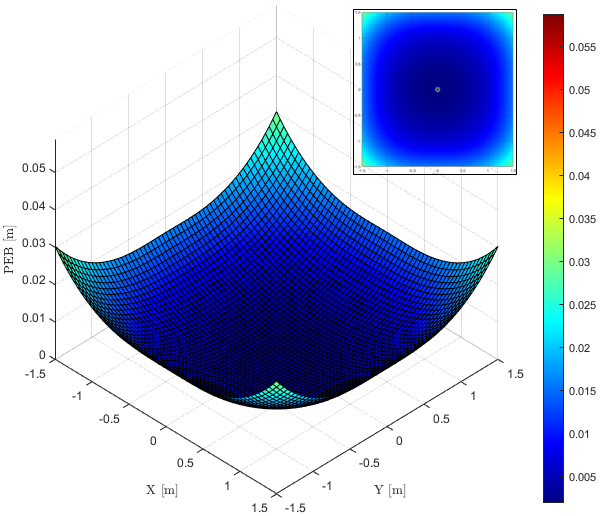
\includegraphics[width=\linewidth]{Figures/IV. Optimization/PEB_K5_optimal.PNG}
    \caption{}
    \label{fig:1a}
  \end{subfigure}
  
  \vspace{1em}  % separación vertical opcional
  
  % Segunda subfigura (b)
  \begin{subfigure}[b]{\columnwidth}
    \centering
    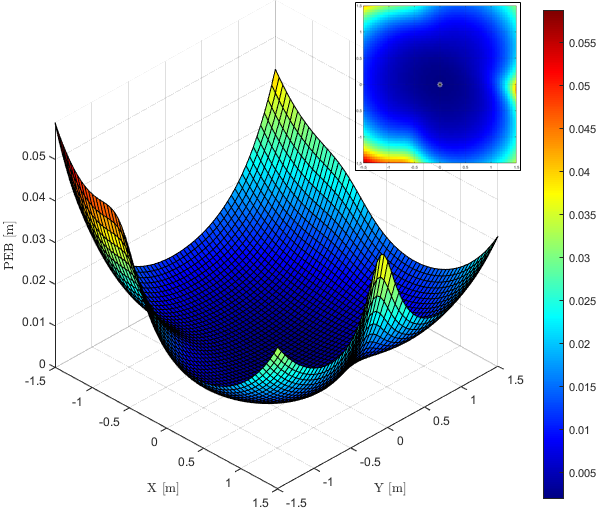
\includegraphics[width=\linewidth]{Figures/IV. Optimization/PEB_K5_random.PNG}
    \caption{}
    \label{fig:1b}
  \end{subfigure}
  
  \caption{Mapa de calor del PEB de la estimación de la posición del receptor dentro de un testbed de 3x3 a una altura de 0.8m con un set de 5-orientaciones (a) set optimo (b) set random.}
  \label{fig:optimo_vs_random_3D}
\end{figure}


La figura \ref{fig:PEB_vs_K} muestra el comporamiento del 90-percentil del CDF del PEB ($\mathrm{PEB}_{90\%}$) del set-optimo de K-orientaciones en 3 diferentes escenarios de potencia de angulo medio ($\Phi_{1/2}$) a un $\mathrm{SNR^*=14dB}$. En todos los escenarios se puede notar que conforme el número de orientaciones aumenta se reduce el $\mathrm{PEB}_{90\%}$. Un trade-off entre la latencia, complejidad y $\mathrm{PEB}_{90\%}$ se encuentra en K=5. Asimismo, con $\Phi_{1/2}=30^\circ$ se requiere al menos 4 orientaciones debido a que la directividad es mayor y 3 orientaciones no proveen la cobertura en el testbed, con 4 a más orientaciones el resultado supera a sus competidores; mientras que $\Phi_{1/2}=45^\circ$ presenta resultados de error competitivos desde K=3, además es ampliamente más usado en aplicacioens comerciales, por lo que, se empleará en las siguientes simulaciones.

\begin{figure}[tb]
    \centering
    
\includegraphics[width=\linewidth]{Figures/IV. Optimization/PEB vs K with theta_half.png}
  \caption{Desempeño del algoritmo con diferente número de orientaciones en 3 escenarios de $\Phi_{1/2}$.}
    \label{fig:PEB_vs_K}
\end{figure}




\begin{figure}[tb]
    \centering
    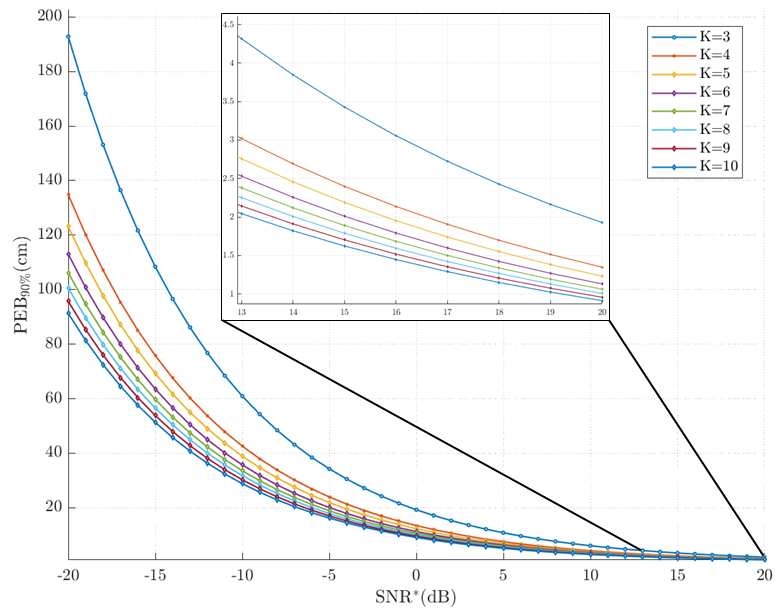
\includegraphics[width=\linewidth]{Figures/IV. Optimization/PEB vs noise (SNR).png}
  \caption{Comportamiento del PEB con respecto a cambios en el SNR.}
    \label{fig:PEB_vs_noise}
\end{figure}

La figura \ref{fig:PEB_vs_noise} muestra el comportamiento del $\mathrm{PEB}_{90\%}$ ante cambios en el SNR con diferentes set-optimos de K-orientacioens. El error dismuneye con el aumento del SNR; mientras que en un mismo SNR el aumento de número de orientacioens disminuye el PEB, el cual se va estrechando conforme se aumenta el SNR.



% *******************************************
\section{Estimador no lineal}
\label{sec:NoLineal}
% *******************************************

Asimismo, se sabe que la potencia óptica colectada por el receptor depende directamente de la posición relativa de éste con respecto a la fuente óptica, en particular a través de los parámetros de distancia $d$, de ángulo de irradiancia $\phi_{t,i}$ y de ángulo de incidencia $\psi_{r}$.

Denotando \(\mathbf{n}_r = [\alpha, \beta, \gamma]\), se observa que:

\begin{equation}
\cos\psi_{r}= \mathbf{n}_r \cdot \mathbf{-n}_{d}
= -\;\frac{\alpha x + \beta y + \gamma (z-H)}{d}.
\label{eq:cos_psi_cartesian}
\end{equation}


Donde $x,y,z$ son las coordenadas del receptor, $H$ es la altura del transmisor. Por tanto, usando \ref{eq:cosenos},  \ref{eq:cos_psi_cartesian} y la relación $d = \sqrt{x^2 + y^2 + (z-H)^2}$ en \ref{eq:received_power} y luego sustituyendo el resultado en \ref{eq:promedios}, se deduce que:

\begin{equation}
P_{o,r}^{(i)} = -\; C \; \frac{(a_i x + b_i y + c_i (z-H))^m}{[x^2 + y^2 + (z-H)^2]^{\frac{m+3}{2}}}
\;(\alpha x + \beta y + \gamma (z-H))+ n. 
\label{eq:nolineal_problem}
\end{equation}



Se observa, por tanto, que las potencias observadas se relacionan directamente con los parámetros a estimar, es decir las coordenadas $\mathbf{R}=(x,y,z)$ del receptor, pero de forma no lineal. Para buscar el vector dirección $\mathbf{n_d}$ en lugar de las coordenadas $\mathbf{R}$, se debe imponer la restricción $x^2 + y^2 + (z-H)^2 = 1$. La ecuación \ref{eq:nolineal_problem} puede reformularse entonces como:

\begin{equation}
    P_{o,r}^{(i)}=-\;C\,Q_i^m(x,y,z)\,L(x,y,z)+ n,
\end{equation}

con \(n\sim\mathcal{N}(0,\sigma^2/N)\) y:

\begin{equation}
Q_i(x,y,z) = a_i x + b_i y + c_i (z-H),
\label{eq:Q}
\end{equation}

\begin{equation}
L(x,y,z) = \alpha x + \beta y + \gamma (z-H).   
\label{eq:L}
\end{equation}


Nos encontramos aquí ante un caso típico de la teoría de la estimación, donde las observaciones promedio $(P_{o,r}^{(i)})$ para diferentes orientaciones $i$ están unidas no linealmente a los parámetros a estimar y contaminadas por ruido gaussiano de densidad conocida. Se sabe que en este contexto no existe un estimador eficiente, pero sí puede hallarse un estimador MVU.

Para ello se resuelve el problema de mínimos cuadrados no lineales minimizando la función de coste \(F(x,y,z)\) definida como:

\begin{equation}
    F(x,y,z)=\sum_{i=1}^{K} F_i(x,y,z),
    \label{eq:fun_cost}
\end{equation}

con:

\begin{equation}
F_i(x,y,z)=(P_{o,r}^{(i)} - (-C)\;Q_i(x,y,z)\,L(x,y,z))^{2}.
\label{eq:fun_cost_explicit}
\end{equation}



Cabe señalar que, puesto que buscamos la estimación de la dirección $\mathbf{n}_{d}$, las coordenadas $x,y,(z-H)$ resultantes de este problema de mínimos cuadrados han de pertenecer a la esfera unitaria \(\mathbb{S}^2\) y garantizar que los polinomios \(Q_i(x,y,z)\) y \(L(x,y,z)\) sean, respectivamente, positivos (pues iguales a \(\cos\phi_i\), con \(0\le\phi_{t,i}\le\pi/2\)) y negativos (pues iguales a \(-\cos\psi_r\), con \(0\le\psi_r\le\pi/2\)).

En otras palabras, buscamos una estimación $\hat{\mathbf{n}}_d$ del vector unitario ${\mathbf{n}}_d$, apuntando de la fuente óptica al receptor, que sea solución del problema de mínimos cuadrados no lineales:

\begin{equation}
\hat{\mathbf{n}}_{d,\mathrm{NL}}=\arg\min_{(x,y,z-H)\in\mathbb{S}^2}F(x,y,z).
\end{equation}


con $F(x,y,z)$ definido en \ref{eq:fun_cost}-\ref{eq:fun_cost_explicit} y $Q_i$, $L$ según \ref{eq:Q}-\ref{eq:L}, sujeto a las restricciones:

\begin{equation}
\begin{aligned}
x^2 + y^2 + (z-H)^2 &= 1, \\
\forall\,i\in\{1,\dots,K\},\quad Q_i(x,y,z) &\ge 0, \\
L(x,y,z) &\le 0.
\end{aligned}
\end{equation}


En la práctica, este problema puede resolverse en \textsc{MATLAB} mediante la función \texttt{solve}, que para este tipo de optimización no lineal recurre internamente a \texttt{fmincon} e implementa métodos de descenso de gradiente.




% *******************************************
\section{Lineal estimator}
\label{sec:Lineal}
% *******************************************

The present section develops the first stage with full mathematical
rigour and presents two statistically grounded estimators:
(i)~generalised least squares (GLS), which is minimum-variance under
Gaussian noise with known covariance, and
(ii)~weighted least squares (WLS), an inexpensive
approximation that neglects the weak cross–correlation between
equations.



%-------------------------------------------------------------------------------
\subsection{Direction Estimation via GLS}
\label{subsec:gls_direction}
%-------------------------------------------------------------------------------

This subsection consolidates the analytical pipeline that converts the raw optical powers into a closed-form, statistically efficient estimate of the direction vector $\mathbf{n}_d$. The exposition proceeds from the determin\-istic constraints, through a rigorous stochastic characterisation of the residuals, to the final GLS solution.

\subsubsection{Lambertian power ratios and homogeneous constraints}
Let $\mu_i=\mathbb E\!\bigl[P_r^{(i)}\bigr]$ be the noise-free power at
orientation~$i$. We define power ratio $\beta$ as:
\begin{equation}
  \beta_i=\bigl(\mu_i/\mu_1\bigr)^{1/m}, \quad i=2,\ldots,K,
  \label{eq:beta_def_gls}
\end{equation}
and, from eq.(\ref{eq:received_power}), (\ref{eq:h_los}) and (\ref{eq:cosenos}), 
$\mu_i\!\propto\!\bigl(\mathbf d\cdot\mathbf n_t^{(i)}\bigr)^{m}$,
each $\beta_i$ imposes
\begin{equation}
  \mathbf d \cdot
  \bigl(\mathbf n_t^{(i)}-\beta_i\mathbf n_t^{(1)}\bigr)=0,
  \quad
  i=2,\ldots,K.
  \label{eq:homog_gls}
\end{equation}
Denoting
$\mathbf a_i\!=\!
 \mathbf n_t^{(i)}-\beta_i\mathbf n_t^{(1)}$,~\eqref{eq:homog_gls}
reads $\mathbf a_i\cdot\mathbf d=0$ and supplies $K-1$ homogeneous hyperplanes that intersect at the true~$\mathbf d$.

\subsubsection{Stochastic perturbation of the ratios}
Let $\smash{P_{r,k}^{(i)}}$ denote the $k$-th noisy observation gathered
while the LED points along $\mathbf n_t^{(i)}$,
$1\!\le k\!\le N$, $1\!\le i\!\le K$.
According to~\eqref{eq:received_power},
$P_{r,k}^{(i)}=\mu_i+\eta_i$ with
$\eta_i\sim\mathcal N(0,\sigma^{2})$ i.i.d.
The sample mean
\[
\hat\mu_i=\frac1N\sum_kP_{r,k}^{(i)}
 \sim\mathcal N(\mu_i,\sigma^{2}/N)
\]
is the MVU estimator.
Injecting $\hat\mu_i$ into~\eqref{eq:beta_def_gls} yields
\[
  \hat\beta_i
  =g_i(\hat\mu_1,\hat\mu_i),
  \qquad
  g_i(x_1,x_2)=\bigl(\frac{x_2}{x_1}\bigr)^{\frac{1}{m}}.
\]
A first-order Taylor expansion of $g_i$ centred at
$\boldsymbol\mu_i=(\mu_1,\mu_i)^{\mathsf T}$ gives
\begin{equation}
  \hat\beta_i
  \approx
  \bar\beta_i
  +\frac{\bar\beta_i}{m}
   \!\left(\frac{\eta_i}{\mu_i}-\frac{\eta_1}{\mu_1}\right),
  \quad
  \bar\beta_i=(\mu_i/\mu_1)^{1/m}.
  \label{eq:beta_lin_gls}
\end{equation}
Hence every $\hat\beta_i$ shares the common perturbation~$\eta_1$,
producing correlation across orientations.

Define the ratio error
$\tilde\eta_i=\hat\beta_i-\bar\beta_i$.  Using~\eqref{eq:beta_lin_gls}
and the independence of $\eta_i$ and $\eta_1$,
\begin{align}
  \operatorname{Var}[\tilde\eta_i]
  &=
  \frac{\sigma^{2}}{Nm^{2}}\,
  \bar\beta_i^{2}\bigl(\mu_i^{-2}+\mu_1^{-2}\bigr),
  \label{eq:var_beta_gls}\\
  \operatorname{Cov}[\tilde\eta_i,\tilde\eta_j]
  &=
  \frac{\sigma^{2}}{Nm^{2}}\,
  \bar\beta_i\bar\beta_j\,\mu_1^{-2},
  \quad i\neq j.
  \label{eq:cov_beta_gls}
\end{align}
The factor $(\mu_i^{-2} + \mu_1^{-2})$ in~\eqref{eq:var_beta_gls}
demonstrates that the variance of $\tilde\eta_i$ depends explicitly on
$\mu_i$, even though each $\eta_k^{(i)}$ has the same variance
$\sigma^2$.  In other words, a single‐LED system exhibits
\emph{heteroscedastic} ratio errors.

\subsubsection{Residuals and their covariance.}
Substituting $\hat\beta_i$ into $\mathbf a_i$,
\(
  \mathbf a_i
   =\bar{\mathbf a}_i-\mathbf n_t^{(1)}\tilde\eta_i,
\)
and taking the inner product with~$\mathbf d$ gives the residual
\[
  r_i
  =\mathbf a_i \cdot \mathbf d
  =\kappa\,\tilde\eta_i,
  \quad
  \kappa=\mathbf n_t^{(1)}\!\cdot\mathbf d.
\]
Consequently, vector of residuals
$\mathbf r=[r_2,\dots,r_n]^{\mathsf T}$ is
zero-mean Gaussian with covariance
$\Sigma_r=\kappa^{2}\Sigma_\beta$,

\[
  \mathbf r \;=\; A^{\mathsf T}\mathbf d \;+\;\boldsymbol\varepsilon,
  \quad
  \boldsymbol\varepsilon \sim \mathcal N\bigl(\mathbf0,\Sigma_r\bigr),
\]

where $\Sigma_\beta$ gathers
\eqref{eq:var_beta_gls}–\eqref{eq:cov_beta_gls}.
Higher-order remainders decay as
$O(\sigma^{4}/N^{2})$ and are negligible for
$\mathrm{SNR}\!\ge\!10$\,dB and $N\!\ge\!50$.



\subsubsection{GLS formulation and closed-form solution}
Collect the normals as
$A=[\mathbf a_2\;\dots\;\mathbf a_n]\in\mathbb R^{3\times(n-1)}$.
With $\Sigma_r$ known, the generalised least-squares problem is
\[
  \hat{\mathbf d}
  =\arg\min_{\|\mathbf d\|=1}
     \mathbf d^{\mathsf T}
     \bigl(A\Sigma_r^{-1}A^{\mathsf T}\bigr)\mathbf d,
\]
whose minimiser is the unit eigenvector associated with the
smallest eigenvalue of
$
  M_{\text{GLS}}
  =A\Sigma_r^{-1}A^{\mathsf T}.
$
In practice, all multiplicative constants in $\Sigma_r^{-1}$ can be
omitted and absorbed into a normalisation of the weight matrix,
since only the eigenvector direction matters. Formally,
\begin{equation}
    \hat{\mathbf{n}}_{d,\rm GLS}
    =\frac{\mathbf v_{\min}\bigl(M_{\text{GLS}}\bigr)}{||\mathbf v_{\min}\bigl(M_{\text{GLS}}\bigr)||}
  \label{eq:gls_dir_final}
\end{equation}
and the sign of $\hat{\mathbf{n}}_{d,\rm GLS}$ is chosen so that
$\hat{\mathbf{n}}_{d,\rm GLS}\cdot\mathbf n_t^{(1)}>0$,
ensuring the vector points from the transmitter towards the receiver.
This estimator is the minimum-variance, unbiased
linear estimator (BLUE) for the linearised model.

%-------------------------------------------------------------------------------
\subsection{WLS as a practical simplification}
%-------------------------------------------------------------------------------

The inversion of $\Sigma_r$ requires an $(n-1)\!\times\!(n-1)$
Cholesky factorisation.  For real-time, low-power receivers a lighter
alternative is attractive.
Neglecting the off-diagonal terms in~\eqref{eq:cov_beta_gls} gives the 
diagonal weight matrix
\[
\tilde\Sigma_r
  =\operatorname{diag}\!\Bigl\{
       \bar\beta_i^{2}\bigl(\mu_i^{-2}+\mu_1^{-2}\bigr)
     \Bigr\}_{i=2}^{n}.
\]
Setting $\mathrm{W}=\tilde\Sigma_r^{-1}$ leads to the WLS cost
\[
  J_{\text{WLS}}(\mathbf d)
  =
  \mathbf d^{\mathsf T}
  \Bigl(A\mathrm{W}A^{\mathsf T}\Bigr)\mathbf d,
  \qquad\|\mathbf d\|=1,
\]
whose minimiser is
\begin{equation}
  \hat{\mathbf{n}}_{d,\rm WLS}
   =\frac{\mathbf v_{\min}\!\bigl(A\mathrm{W}A^{\mathsf T}\bigr)}{||\mathbf v_{\min}\!\bigl(A\mathrm{W}A^{\mathsf T}\bigr)||}.
  \label{eq:WLS_solution}
\end{equation}

The neglected off‐diagonal covariance terms scale as
$\mu_1^{-2}$, whereas the diagonal entries scale as
$\mu_i^{-2}+\mu_1^{-2}$.  When the reference orientation $(i=1)$
satisfies $\mu_1\gg\mu_i$ for most $i$, one obtains
$\mu_1^{-2}\ll\mu_i^{-2}$, so that the off‐diagonal terms are at least
20 dB below the diagonal terms.  In such regimes, the WLS estimator
captures over 95\% of the statistical efficiency of GLS while avoiding
matrix inversions.  In contrast, in nearly symmetric geometries where
$\mu_i\approx\mu_1$ for many $i$, off‐diagonal correlations become
important and the full GLS should be used for optimal performance.



%-------------------------------------------------------------------------------
% Algorithm - 3-D position estimator
%-------------------------------------------------------------------------------
\begin{algorithm}[tb]
  \caption{3-D Position Estimation from $n$ Orientations}
  \label{alg:position}
  \small
  \begin{algorithmic}[1]
  \Require
    \begin{tabular}[t]{@{}l@{}}
      Power samples $P_{r,k}^{(i)}$ ($k=1,\dots,N$, $i=1,\dots,K$);\\
      steering vectors $\mathbf n_t^{(i)}$; Lambertian order $m$;\\
      noise variance $\sigma^{2}$; \textsc{mode}$\in\{\mathrm{GLS},\mathrm{WLS}\}$;\\
      radiometric constant $C$.
    \end{tabular}
  \Ensure
    $\hat{\mathbf R}$ (3-D position of the receiver)
  \Statex
  \State {\bfseries Direction finding:}
  \State \quad Compute $\hat\mu_i=\tfrac{1}{N}\sum_{k=1}^N P_{r,k}^{(i)}$
            for $i=1,\dots,K$
  \State \quad Compute $\hat\beta_i=(\hat\mu_i/\hat\mu_1)^{1/m}$ for $i=2,\dots,K$
  \State \quad Form $\mathbf a_i = \mathbf n_t^{(i)} - \hat\beta_i\,\mathbf n_t^{(1)}$
  \State \quad Set $A = [\mathbf a_2,\dots,\mathbf a_n]$
  \If{\textsc{mode} = GLS}
    \State \quad Build $\Sigma_r$ via
           \eqref{eq:var_beta_gls}--\eqref{eq:cov_beta_gls},
           substituting $\beta_i \leftarrow \hat\beta_i$
    \State \quad $M \gets A\,\Sigma_r^{-1}\,A^{\mathsf T}$
  \Else\Comment{WLS (diagonal approximation)}
    \State \quad $\tilde\Sigma_r \gets 
           \operatorname{diag}\bigl\{\hat\beta_i^{2}\bigl(\hat\mu_i^{-2}+\hat\mu_1^{-2}\bigr)\bigr\}$
    \State \quad $M \gets A\,\tilde\Sigma_r^{-1}\,A^{\mathsf T}$
  \EndIf
  \State \quad Compute $\mathbf v_{\min} =$ eigenvector of $M$ with smallest eigenvalue
  \State \quad $\hat{\mathbf n}_d \gets \mathbf v_{\min}/\|\mathbf v_{\min}\|$
  \If{$\hat{\mathbf n}_d\cdot\mathbf n_t^{(1)} < 0$}
    \State \quad $\hat{\mathbf n}_d \gets -\,\hat{\mathbf n}_d$ \Comment{Ensure pointing to Rx}
  \EndIf

  \Statex
  \State {\bfseries Distance Estimation (beamsteering):}
  \State \quad Set $\mathbf n_t \gets \hat{\mathbf n}_d$,\quad $\mathbf n_r \gets -\,\hat{\mathbf n}_d$
  \State \quad Collect $N$ power samples $P_r^{*(k)}$ 
  \State \quad Compute $\hat\mu^* = \tfrac{1}{N}\sum_{k=1}^{N} P_{r,k}^*$
  \State \quad $\hat d \gets \sqrt{\tfrac{C}{\hat\mu^*}}$

  \Statex
  \State {\bfseries Final 3-D position:}
  \State \quad $\hat{\mathbf R} \gets \mathbf T + \hat d \,\hat{\mathbf n}_d$
  \State \Return $\hat{\mathbf R}$
  \end{algorithmic}
\end{algorithm}





\begin{figure}[htb]
    \centering
    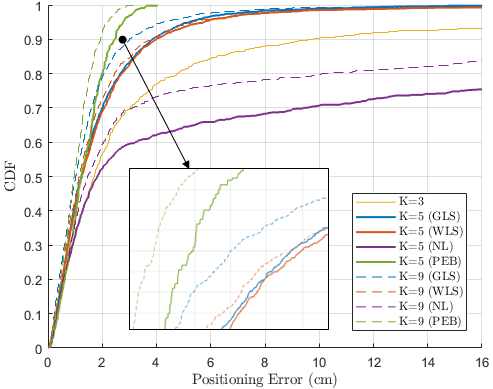
\includegraphics[width=\linewidth]{Figures/VII.Simulations/figCDF.png}
    \caption{Comparación de CDF de diferentes métodos y $K$.}
    \label{fig:CDF}
\end{figure}




% *******************************************
\section{Results}
\label{sec:results}
% *******************************************

En la Figura \ref{fig:CDF} se muestra el CDF del error de estimación de la posición por cada uno de los métodos presentados previamente, empleando un set de K-orientaciones para $K=5$ y $9$. Como se puede apreciar el método GLS presenta un desempeño comparable con el método NL y cercanos al PEB; mientras que el WLS presenta un mayor error pero es de menor complejidad, lo que impacta en la latencia.




La Figura \ref{fig:latency} muestra una comparativa entre el CDF del error al 90\% ($e_{90\%})$ de los diferente métodos y la latencia, para los escenarios de $K=5$ y $9$. Como se puede apreciar el método NL presenta una mayor latencia debido a que es un método que recurre iterativamente a la busqueda de la solución; mientras que los otros métodos GLS y WLS son soluciones cerradas.

\begin{figure}[htb]
    \centering
    
\includegraphics[width=\linewidth]{Figures/VII.Simulations/latency.png}
    \caption{Latencia de los diferentes métodos.}
    \label{fig:latency}
\end{figure}

La Figura \ref{fig:estimation} muestra la estimación de la posición del receptor por el método WLS y GLS con $K=5$ en 3 diferentes alturas $h (0, 0.6, 1.2)$ y la referencia de la posición real. Como se puede apreciar cuando $h=1.2$ el error aumenta conforme estamos en los extremos especialmente en las esquinas debido a que se tiene menor SNR por los angulos extremos que forma con los vectores de orientación; mientras que en $h=0$ la estimación es mas uniforme. 

\begin{figure}[htb]
    \centering
    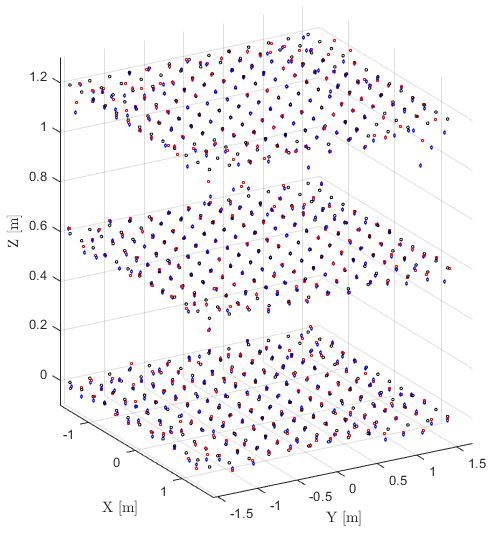
\includegraphics[width=\linewidth]{Figures/VII.Simulations/estimation_3D.png}
    \caption{Estimacion de la posicion en 3D para 3 diferentes niveles de altura considerando $K=5$ orientaciones. GLS de azul, WLS de rojo, References de negro.}
    \label{fig:estimation}
\end{figure}


\end{document}